% Options for packages loaded elsewhere
\PassOptionsToPackage{unicode}{hyperref}
\PassOptionsToPackage{hyphens}{url}
\PassOptionsToPackage{dvipsnames,svgnames,x11names}{xcolor}
%
\documentclass[
]{agujournal2019}

\usepackage{amsmath,amssymb}
\usepackage{iftex}
\ifPDFTeX
  \usepackage[T1]{fontenc}
  \usepackage[utf8]{inputenc}
  \usepackage{textcomp} % provide euro and other symbols
\else % if luatex or xetex
  \usepackage{unicode-math}
  \defaultfontfeatures{Scale=MatchLowercase}
  \defaultfontfeatures[\rmfamily]{Ligatures=TeX,Scale=1}
\fi
\usepackage{lmodern}
\ifPDFTeX\else  
    % xetex/luatex font selection
\fi
% Use upquote if available, for straight quotes in verbatim environments
\IfFileExists{upquote.sty}{\usepackage{upquote}}{}
\IfFileExists{microtype.sty}{% use microtype if available
  \usepackage[]{microtype}
  \UseMicrotypeSet[protrusion]{basicmath} % disable protrusion for tt fonts
}{}
\makeatletter
\@ifundefined{KOMAClassName}{% if non-KOMA class
  \IfFileExists{parskip.sty}{%
    \usepackage{parskip}
  }{% else
    \setlength{\parindent}{0pt}
    \setlength{\parskip}{6pt plus 2pt minus 1pt}}
}{% if KOMA class
  \KOMAoptions{parskip=half}}
\makeatother
\usepackage{xcolor}
\setlength{\emergencystretch}{3em} % prevent overfull lines
\setcounter{secnumdepth}{5}
% Make \paragraph and \subparagraph free-standing
\ifx\paragraph\undefined\else
  \let\oldparagraph\paragraph
  \renewcommand{\paragraph}[1]{\oldparagraph{#1}\mbox{}}
\fi
\ifx\subparagraph\undefined\else
  \let\oldsubparagraph\subparagraph
  \renewcommand{\subparagraph}[1]{\oldsubparagraph{#1}\mbox{}}
\fi


\providecommand{\tightlist}{%
  \setlength{\itemsep}{0pt}\setlength{\parskip}{0pt}}\usepackage{longtable,booktabs,array}
\usepackage{calc} % for calculating minipage widths
% Correct order of tables after \paragraph or \subparagraph
\usepackage{etoolbox}
\makeatletter
\patchcmd\longtable{\par}{\if@noskipsec\mbox{}\fi\par}{}{}
\makeatother
% Allow footnotes in longtable head/foot
\IfFileExists{footnotehyper.sty}{\usepackage{footnotehyper}}{\usepackage{footnote}}
\makesavenoteenv{longtable}
\usepackage{graphicx}
\makeatletter
\def\maxwidth{\ifdim\Gin@nat@width>\linewidth\linewidth\else\Gin@nat@width\fi}
\def\maxheight{\ifdim\Gin@nat@height>\textheight\textheight\else\Gin@nat@height\fi}
\makeatother
% Scale images if necessary, so that they will not overflow the page
% margins by default, and it is still possible to overwrite the defaults
% using explicit options in \includegraphics[width, height, ...]{}
\setkeys{Gin}{width=\maxwidth,height=\maxheight,keepaspectratio}
% Set default figure placement to htbp
\makeatletter
\def\fps@figure{htbp}
\makeatother
% definitions for citeproc citations
\NewDocumentCommand\citeproctext{}{}
\NewDocumentCommand\citeproc{mm}{%
  \begingroup\def\citeproctext{#2}\cite{#1}\endgroup}
\makeatletter
 % allow citations to break across lines
 \let\@cite@ofmt\@firstofone
 % avoid brackets around text for \cite:
 \def\@biblabel#1{}
 \def\@cite#1#2{{#1\if@tempswa , #2\fi}}
\makeatother
\newlength{\cslhangindent}
\setlength{\cslhangindent}{1.5em}
\newlength{\csllabelwidth}
\setlength{\csllabelwidth}{3em}
\newenvironment{CSLReferences}[2] % #1 hanging-indent, #2 entry-spacing
 {\begin{list}{}{%
  \setlength{\itemindent}{0pt}
  \setlength{\leftmargin}{0pt}
  \setlength{\parsep}{0pt}
  % turn on hanging indent if param 1 is 1
  \ifodd #1
   \setlength{\leftmargin}{\cslhangindent}
   \setlength{\itemindent}{-1\cslhangindent}
  \fi
  % set entry spacing
  \setlength{\itemsep}{#2\baselineskip}}}
 {\end{list}}
\usepackage{calc}
\newcommand{\CSLBlock}[1]{\hfill\break\parbox[t]{\linewidth}{\strut\ignorespaces#1\strut}}
\newcommand{\CSLLeftMargin}[1]{\parbox[t]{\csllabelwidth}{\strut#1\strut}}
\newcommand{\CSLRightInline}[1]{\parbox[t]{\linewidth - \csllabelwidth}{\strut#1\strut}}
\newcommand{\CSLIndent}[1]{\hspace{\cslhangindent}#1}

\usepackage{url} %this package should fix any errors with URLs in refs.
\usepackage{lineno}
\usepackage[inline]{trackchanges} %for better track changes. finalnew option will compile document with changes incorporated.
\usepackage{soul}
\linenumbers
\makeatletter
\@ifpackageloaded{caption}{}{\usepackage{caption}}
\AtBeginDocument{%
\ifdefined\contentsname
  \renewcommand*\contentsname{Table of contents}
\else
  \newcommand\contentsname{Table of contents}
\fi
\ifdefined\listfigurename
  \renewcommand*\listfigurename{List of Figures}
\else
  \newcommand\listfigurename{List of Figures}
\fi
\ifdefined\listtablename
  \renewcommand*\listtablename{List of Tables}
\else
  \newcommand\listtablename{List of Tables}
\fi
\ifdefined\figurename
  \renewcommand*\figurename{Figure}
\else
  \newcommand\figurename{Figure}
\fi
\ifdefined\tablename
  \renewcommand*\tablename{Table}
\else
  \newcommand\tablename{Table}
\fi
}
\@ifpackageloaded{float}{}{\usepackage{float}}
\floatstyle{ruled}
\@ifundefined{c@chapter}{\newfloat{codelisting}{h}{lop}}{\newfloat{codelisting}{h}{lop}[chapter]}
\floatname{codelisting}{Listing}
\newcommand*\listoflistings{\listof{codelisting}{List of Listings}}
\makeatother
\makeatletter
\makeatother
\makeatletter
\@ifpackageloaded{caption}{}{\usepackage{caption}}
\@ifpackageloaded{subcaption}{}{\usepackage{subcaption}}
\makeatother
\ifLuaTeX
  \usepackage{selnolig}  % disable illegal ligatures
\fi
\usepackage{bookmark}

\IfFileExists{xurl.sty}{\usepackage{xurl}}{} % add URL line breaks if available
\urlstyle{same} % disable monospaced font for URLs
\hypersetup{
  pdftitle={T is for Topology},
  pdfauthor={Tanya Strydom; Andrew P. Beckerman},
  pdfkeywords={food web, network construction},
  colorlinks=true,
  linkcolor={blue},
  filecolor={Maroon},
  citecolor={Blue},
  urlcolor={Blue},
  pdfcreator={LaTeX via pandoc}}

\journalname{Some fancy journal}

\draftfalse

\begin{document}
\title{T is for Topology}

\authors{Tanya Strydom\affil{1}, Andrew P. Beckerman\affil{1}}
\affiliation{1}{University of Sheffield, }
\correspondingauthor{Tanya Strydom}{t.strydom@sheffield.ac.uk}


\begin{abstract}
Pending\ldots{}
\end{abstract}

\section*{Plain Language Summary}
We want to know a bit more about the different network topology
generators (predict tools) and how they differ - \emph{i.e.,} their
strengths and weaknesses



\section{Introduction}\label{introduction}

The standard run of the mill that we cannot always feasibly construct
networks because 1. hard, 2. time (yay dinosaurs, but also the future
and impending doom I guess), and 3. probably something else meaningful
that's just slipping my mind at the moment. Some of the usual culprits
will come in here like: Jordano (2016b); (Jordano, 2016a); Poisot et al.
(2021)

\begin{quote}
TODO: standardise language between a topology generator and a topology
predictor\ldots{} I guess they can both be considered models but I'm not
quite sure\ldots{}
\end{quote}

\subsection{Philosophical contemplation when constructing interaction
networks}\label{philosophical-contemplation-when-constructing-interaction-networks}

\subsubsection{Why do we want to construct an interaction
network?}\label{why-do-we-want-to-construct-an-interaction-network}

Arguably the need for methods and tools for constructing interaction
networks arises from two different (but still aligned) places of
interest within the field of network ecology. On the one side of the
spectrum sits the researcher who is interested in generating a set of
ecologically plausible but not necessarily realised `in the field' for
the purpose of running further simulations (\emph{e.g.,} extinction sim
REF? \textbf{TODO}) or understanding some higher-level process
(\emph{e.g.,} energetics REF \textbf{TODO}). This researcher is
contrasted by one that is interested in constructing real-world,
location specific interactions networks in lieu of having access to data
generated in the field (see Strydom et al. (2021) for a discussion on
this). Of course these two categories are not distinct, mutually
exclusive, groups but can rather be viewed as operating on a gradient
ranging from a need for generality (\emph{something}) to a need for
specificity (local-level predictions) when it comes to the quality(?) of
the network that is constructed by a specific tool. Of course this
research need would also reflected in the model development process
itself and thus the idea of what a `good enough' constructed network
will be in the context of assessing the performance of a specific model.

Joel E. Cohen et al. (1985) states that \emph{``{[}Their{]} approach is
more like gross anatomy than like physiology\ldots{} that is, the gross
anatomy is frozen, rather than in motion.''}.

Interestingly Williams \& Martinez (2008) also explicitly talk about
\emph{structural} food-web models in their introduction\ldots{} so how I
see it that means that there has always been this inherent
acknowledgement that models are function at a specific `network level'.

\subsubsection{The history behind the
approach}\label{the-history-behind-the-approach}

Maybe a brief history of the development of predictive tools/topo
generators? Sort of where the theory/body of work was based and how that
has changed? IS there a difference between topo generator and predictive
tool - I'm inclined to think that it aligns with the whole debate of
high level structure vs node-level perfection

Maybe start here with discussing the core mechanistic differences that
models will work at --- some are really concerned about (and thus
constrained by) structure, others are more mechanistic in nature
\emph{i.e.,} species \emph{a} has the capacity to eat species \emph{b}
because traits (read gob size), and then you get Rohr et al. (2010) and
Strydom et al. (2022) that sit in the weird liminal latent space\ldots{}

Here I will probably get on my (newly discovered) soapbox and wax
lyrical about how in certain situations structure is enough (and that
will probably be for some high-level things like thinking about energy
flows etc., I can also see a world in which maybe you want to do some
sort of robustness/extinction work - since then you're usually doing
`random' (within limits) extinctions) but there may be use cases where
we are really interested in the node-level interactions \emph{i.e.,}
species identity is like a thing we need to care about and also be able
to retrieve specific interactions at specific nodes correctly. What is
the purpose of generating a network? Is it an element of a bigger
question we are asking, \emph{e.g.,} I want to generate a series of
networks to do some extinction simulations/bioenergetic stuff OR are we
looking for a `final product' network that is relevant to a specific
location? (this can still be broad in geographic scope).

At some point we are going to need to discuss the key differences and
implications between predicting a metaweb (\emph{sensu} Jennifer A.
Dunne (2006)) and a network realisation. And here I can't help but think
about Poisot et al. (2015) (and probably other papers) that discuss how
the local factors are going to play a role and even the same pair of
species may interact differently in different points in the landscape.

\begin{quote}
Do we need to delve into individual-based networks? (\emph{sensu} Tinker
2012, Araújo 2008) I think its probably a step too far and one starts
creeping into apples and pears type of comparisons. Especially since
these work off of already existing networks (I seem to recall) and its
more about about `tweaking' those - so not so much \emph{de novo}
predictions. Although this might be useful to keep in mind when it comes
to re-wiring\ldots{} Also on that note do we opn the re-wiring door here
in this ms or wait it out a bit.
\end{quote}

\section{Data \& Methods}\label{sec-data-methods}

\subsection{Overview of models}\label{overview-of-models}

\subsubsection{Structural models}\label{structural-models}

\textbf{Random model} (Erdős \& Rényi, 1959): Links are assembled
randomly, not developed within an ecological framework. But of course
could still hold if we assume that communities are randomly assembled in
terms of who is interacting with who (I seem to think that's sort of
what May was arguing but I would need to remind myself)

\textbf{Cascade model} (Joel E. Cohen et al., 1990): Much like the name
suggests the cascade model rests on the idea that species feed on one
another in a hierarchical manner. This rests on the assumption that the
links within a network are variably distributed across the network; with
the proportion of links decreasing as one moves up the trophic levels
(\emph{i.e.,} `many' prey and `few' predators). This is achieved by
assigning all species a random rank, this rank will then determine both
the predators and prey of that species. A species will have a particular
probability of being fed on by any species with a higher ranking than
it, this probability is constrained by the specified connectance of the
network. Interestingly here `species' are treated as any individual that
consume and are consumed by the same `species', \emph{i.e.,} these are
not taxonomical species (Joel E. Cohen et al., 1985). The original
cascade model has altered to be more `generalised' (Stouffer et al.,
2005), which altered the probability distribution of the prey that could
be consumed by a species.

\textbf{Niche model} (Williams \& Martinez, 2000): The niche model
introduces the idea that species interactions are based on the `feeding
niche' of a species. Broadly, all species are randomly assigned a
`feeding niche' range and all species that fall in this range can be
consumed by that species (thereby allowing for cannibalism). The niche
of each species is randomly assigned and the range of each species'
niche is (in part) constrained by the specified connectance of the
network. The niche model has also been modified, although it appears
that adding to the `complexity' of the niche model does not improve on
its ability to generate a more ecologically `correct' network (Williams
\& Martinez, 2008).

\textbf{Nested hierarchy model} (Cattin et al., 2004):

\subsubsection{Mechanistic models}\label{mechanistic-models}

\textbf{Allometric diet breadth model (ADBM)} (Petchey et al., 2008):

\textbf{Log-ratio} (Rohr et al., 2010): Interestingly often used in
paleo settings (at least that's what it currently looks like in my
mind\ldots{} (\emph{e.g.,} Yeakel et al. (2014), Pires et al. (2020))

\textbf{Stochastic} (Rossberg et al., 2006):

\textbf{PFIM} (Shaw et al., 2024):

\textbf{Trait-based} (Caron et al., 2022):

\textbf{Graph embedding} (Strydom et al., 2023): \emph{e.g.,} (Strydom
et al., 2022)

I know tables are awful but in this case they may make more sense. Also
I don't think I'm at the point where I can say that the table is
complete/comprehensive but it getting there Not sure about putting in
some papers that have used the model - totes happy to drop those I
think\ldots{}

\begin{longtable}[]{@{}llll@{}}
\caption{Lets make a table that gives an overview of the different
topology generators that we will look
at}\label{tbl-history}\tabularnewline
\toprule\noalign{}
Model & Core Mechanism & End product & Data (?) \\
\midrule\noalign{}
\endfirsthead
\toprule\noalign{}
Model & Core Mechanism & End product & Data (?) \\
\midrule\noalign{}
\endhead
\bottomrule\noalign{}
\endlastfoot
random & structural & network & \\
cascade & structural & network & \\
niche & structural & network & \\
nested hierarchical & structural & network & \\
ADBM & mechanistic & \textbf{TODO} & \\
log-ratio & mechanistic & \textbf{TODO} & \\
PFIM & mechanistic & metaweb & \\
graph embedding & mechanistic & metaweb & \\
trait-based & mechanistic & metaweb & \\
stochastic & \textbf{TODO} & \textbf{TODO} & \\
\end{longtable}

\begin{quote}
Might be nice to have a little appendix/supp mat that breaks down the
models in detail so that they are all in one place so that someone (grad
student being told they need to build networks) some day can go and
educate themselves with slightly lower effort. This will also be useful
for me should I end up having to do some actual coding - think of this
as step one in the pseudo code process.
\end{quote}

\subsection{Datasets used}\label{datasets-used}

Here I think we need to span a variety of domains, at minimum aquatic
and terrestrial but maybe there should be a `scale' element as well
\emph{i.e.,} a regional and local network. I think there is going to be
a `turning point' where structural will take over from mechanistic in
terms of performance. More specifically at local scales bioenergetic
constraints (and co-occurrence) may play a bigger role in structuring a
network whereas at the metaweb level then mechanistic may make more
(since by default its about who can potentially interact and obviously
not constrained by real-world scenarios) \emph{sensu} Caron et al.
(2023). Although having said that I feel that contradicts the idea of
backbones (\emph{sensu} Bramon Mora (sp?) et al \& Stouffer et al) But
that might be where we get the idea of core \emph{structure} vs
something like linkage density. So core things like trophic level/chain
length will be conserved but connectance might not (I think I understand
what I'm trying to say here)

I think we should also use the Dunne (I think) Cambrian (also think)
network (I was correct and its this one Jennifer A. Dunne et al.
(2008)). Because 1) it gives the paleo-centric methods their moment in
the sun and 2) I think it also brings up the interesting question of can
we use modern structure to predict past ones? Here one might expect a
more mechanistic approach to shine.

Draw the other datasets from \texttt{Mangal} because they will be nicely
formatted and essentially at point and shoot level

\subsection{Comparing different
models}\label{comparing-different-models}

For now the (still essentially pending) workflow/associated code can be
found at the following repository
\href{https://github.com/BecksLab/topology_generators}{BecksLab/topology\_generators}

\begin{enumerate}
\def\labelenumi{\arabic{enumi}.}
\tightlist
\item
  Shortlist/finalise the different topo generators
\item
  collate/translate into \texttt{Julia}

  \begin{itemize}
  \tightlist
  \item
    \emph{e.g.,} some models wil be in SpeciesInteractionNetworks.jl
    (new EcoNet); I know (parts of) the transfer learning stuff is and
    the niche model
  \item
    others will need to be coded out (the more simpler models should be
    easier)
  \item
    can also consider \texttt{R} but then it becomes a case of porting
    things left and right depending on how we decide to do the post
    analyses
  \end{itemize}
\item
  Curate networks for the different datasets/scenarios we select - I
  feel like there might be some scenarios that we can't do all models
  for all datasets but maybe I'm being a pessimist.

  \begin{itemize}
  \tightlist
  \item
    Need to also think about where one might find the additional data
    for some of the models\ldots{}

    \begin{itemize}
    \tightlist
    \item
      Body size: Herberstein et al. (2022) - Although maybe Andrew has
      strong thotsTM RE the one true body size database to rule them
      all\ldots{}
    \item
      Other trait sources: Wilman et al. (2014) and Jones et al. (2009)
    \item
      This is where we'll get the paleo traits from if I'm correct
      Bambach et al. (2007)
    \item
      Phylogeny stuff: Upham et al. (2019) (what we used for TL but its
      only mammals\ldots) but I'm sure there will be others
    \end{itemize}
  \item
    Also limitation of scope\ldots{} \emph{e.g.,} do we even dare to
    think about including plants/basal producers (see \emph{e.g.,}
    Valdovinos et al. (2023))
  \item
    Taxonomic harmonisation - something to think about and check
  \end{itemize}
\item
  compare model performance based on the ideas currently listed in the
  results section.
\item
  Make a pretty picture that summarises things - maybe overlapping Venn
  circles that showcase which models do well in the different
  spheres/aspects of life
\end{enumerate}

\section{Results}\label{results}

How we want to compare and contrast. I think there won't be a `winner'
and thus we need to think of `tests' that are going to measure
performance in different situations/settings. With that in mind I think
some valuable points to consider would be:

\begin{itemize}
\tightlist
\item
  Structural vs pairwise link predictions (graph vs node level)

  \begin{itemize}
  \tightlist
  \item
    \% of links correctly retrieved
  \item
    connectance
  \item
    trophic level
  \item
    generalism vs specialism
  \item
    something related to false positives/negatives
  \item
    intervality
  \end{itemize}
\item
  Data `cost' (some methods might need a lot lot of supporting data vs
  something very light weight)
\item
  I think it would be remiss to not also take into consideration
  computational cost
\item
  something about the network output - I'm acknowledging my biases and
  saying that probabilistic (or \emph{maybe} weighted) links are the way
\end{itemize}

Joel E. Cohen et al. (1985) actually tells us that the cascade model
only really works for communities that range from 3-33 species\ldots{}
and Williams \& Martinez (2008) also highlights how structural models
really only work for small communities

\begin{quote}
maybe we can put these into broader categories - if we do start doing
the venn overlap thing. \emph{E.g.,} local scale predictions, regional
scale predictions, pairwise interactions, structural (energetics),
computationally cheap, low cost data
\end{quote}

\subsection{Qualitative stuff}\label{qualitative-stuff}

\begin{figure}[H]

\centering{

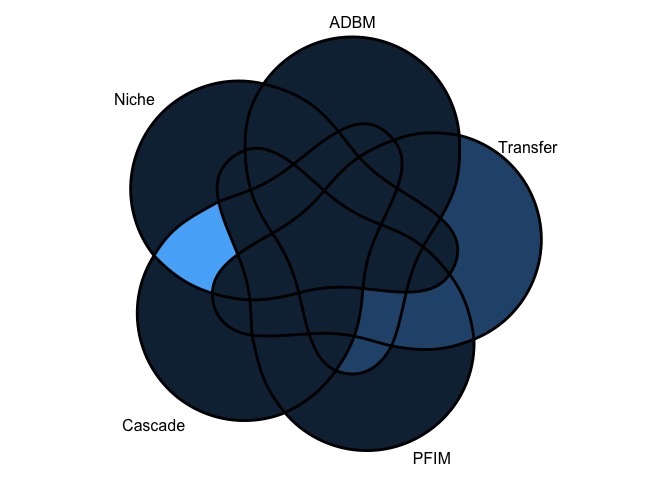
\includegraphics{index_files/figure-latex/notebooks-model_qualitative-fig-venn-output-1.png}

}

\caption{\label{fig-venn}Venn diagram for qualitative analysis/overview
of the fancy maths things}

\end{figure}%

\textsubscript{Source:
\href{https://BecksLab.github.io/ms_t_is_for_topology/index.qmd.html}{Article
Notebook}}

\section{Discussion}\label{discussion}

I think a big take home will (hopefully) be how different approaches do
better in different situations and so you as an end user need to take
this into consideration and pick accordingly. I think Petchey et al.
(2011) might have (and share) some thoughts on this (thanks Andrew). I
feel like I need to look at Berlow et al. (2008) but maybe not exactly
in this context but vaguely adjacent.

An interesting thing to also think about (and arguably it will be
addressed based on some of the other thoughts and ideas) is data
dependant and data independent `parametrisation' of the models\ldots{}

I probably think about this point too much but a point of discussion
that I think will be interesting to bring up the idea that if a model is
missing a specific pairwise link but doing well at the structural level
then when does it matter? I think this is covered with the whole node vs
graph level performance but I kind of just want to bring it up here
again because also one of those things that I think about a bit too much
probably\ldots{}

\begin{quote}
Thinking very long term here and maybe a bit beyond the scope but also
thinking about a multi- model approach? So in other words using one
model to build an initial network but maybe a second one to constrain it
a bit better. I blame this thought on the over-connected PFIM food
webs\ldots{}
\end{quote}

\section*{References}\label{references}
\addcontentsline{toc}{section}{References}

\vspace{1em}

\textsubscript{Source:
\href{https://BecksLab.github.io/ms_t_is_for_topology/index.qmd.html}{Article
Notebook}}

\phantomsection\label{refs}
\begin{CSLReferences}{1}{0}
\bibitem[\citeproctext]{ref-bambachAutecologyFillingEcospace2007}
Bambach, R. K., Bush, A. M., \& Erwin, D. H. (2007). Autecology and the
{Filling} of {Ecospace}: {Key Metazoan Radiations}.
\emph{Palaeontology}, \emph{50}(1), 1--22.
\url{https://doi.org/10.1111/j.1475-4983.2006.00611.x}

\bibitem[\citeproctext]{ref-berlowGoldilocksFactorFood2008}
Berlow, E. L., Brose, U., \& Martinez, N. D. (2008). The {``{Goldilocks}
factor''} in food webs. \emph{Proceedings of the National Academy of
Sciences}, \emph{105}(11), 4079--4080.
\url{https://doi.org/10.1073/pnas.0800967105}

\bibitem[\citeproctext]{ref-caronAddressingEltonianShortfall2022}
Caron, D., Maiorano, L., Thuiller, W., \& Pollock, L. J. (2022).
Addressing the {Eltonian} shortfall with trait-based interaction models.
\emph{Ecology Letters}, \emph{25}(4), 889--899.
\url{https://doi.org/10.1111/ele.13966}

\bibitem[\citeproctext]{ref-caronTrophicInteractionModels2023}
Caron, D., Brose, U., Lurgi, M., Blanchet, G., Gravel, D., \& Pollock,
L. J. (2023, May). Trophic interaction models predict interactions
across space, not food webs. {EcoEvoRxiv}.
\url{https://doi.org/10.32942/X29K55}

\bibitem[\citeproctext]{ref-cattinPhylogeneticConstraintsAdaptation2004}
Cattin, M.-F., Bersier, L.-F., Banašek-Richter, C., Baltensperger, R.,
\& Gabriel, J.-P. (2004). Phylogenetic constraints and adaptation
explain food-web structure. \emph{Nature}, \emph{427}(6977), 835--839.
\url{https://doi.org/10.1038/nature02327}

\bibitem[\citeproctext]{ref-cohenStochasticTheoryCommunity1985}
Cohen, Joel E., Newman, C. M., \& Steele, J. H. (1985). A stochastic
theory of community food webs {I}. {Models} and aggregated data.
\emph{Proceedings of the Royal Society of London. Series B. Biological
Sciences}, \emph{224}(1237), 421--448.
\url{https://doi.org/10.1098/rspb.1985.0042}

\bibitem[\citeproctext]{ref-cohenCommunityFoodWebs1990}
Cohen, Joel E., Briand, F., \& Newman, C. (1990). \emph{Community {Food
Webs}: {Data} and {Theory}}. {Berlin Heidelberg}: {Springer-Verlag}.

\bibitem[\citeproctext]{ref-dunneNetworkStructureFood2006}
Dunne, Jennifer A. (2006). The {Network Structure} of {Food Webs}. In
Jennifer A. Dunne \& M. Pascual (Eds.), \emph{Ecological networks:
{Linking} structure and dynamics} (pp. 27--86). {Oxford University
Press}.

\bibitem[\citeproctext]{ref-dunneCompilationNetworkAnalyses2008}
Dunne, Jennifer A., Williams, R. J., Martinez, N. D., Wood, R. A., \&
Erwin, D. H. (2008). Compilation and {Network Analyses} of {Cambrian
Food Webs}. \emph{PLOS Biology}, \emph{6}(4), e102.
\url{https://doi.org/10.1371/journal.pbio.0060102}

\bibitem[\citeproctext]{ref-erdosRandomGraphs1959}
Erdős, P., \& Rényi, A. (1959). On {Random Graphs I}.
\emph{Publicationes Mathematicae}.
\url{https://doi.org/10.5486/PMD.1959.6.3-4.12}

\bibitem[\citeproctext]{ref-herbersteinAnimalTraitsCuratedAnimal2022}
Herberstein, M. E., McLean, D. J., Lowe, E., Wolff, J. O., Khan, M. K.,
Smith, K., et al. (2022). {AnimalTraits} - a curated animal trait
database for body mass, metabolic rate and brain size. \emph{Scientific
Data}, \emph{9}(1), 265.
\url{https://doi.org/10.1038/s41597-022-01364-9}

\bibitem[\citeproctext]{ref-jonesPanTHERIASpecieslevelDatabase2009}
Jones, K. E., Bielby, J., Cardillo, M., Fritz, S. A., O'Dell, J., Orme,
C. D. L., et al. (2009). {PanTHERIA}: A species-level database of life
history, ecology, and geography of extant and recently extinct mammals.
\emph{Ecology}, \emph{90}(9), 2648--2648.
\url{https://doi.org/10.1890/08-1494.1}

\bibitem[\citeproctext]{ref-jordanoChasingEcologicalInteractions2016}
Jordano, P. (2016a). Chasing {Ecological Interactions}. \emph{PLOS
Biology}, \emph{14}(9), e1002559.
\url{https://doi.org/10.1371/journal.pbio.1002559}

\bibitem[\citeproctext]{ref-jordanoSamplingNetworksEcological2016}
Jordano, P. (2016b). Sampling networks of ecological interactions.
\emph{Functional Ecology}. \url{https://doi.org/10.1111/1365-2435.12763}

\bibitem[\citeproctext]{ref-petcheySizeForagingFood2008}
Petchey, O. L., Beckerman, A. P., Riede, J. O., \& Warren, P. H. (2008).
Size, foraging, and food web structure. \emph{Proceedings of the
National Academy of Sciences}, \emph{105}(11), 4191--4196.
\url{https://doi.org/10.1073/pnas.0710672105}

\bibitem[\citeproctext]{ref-petcheyFitEfficiencyBiology2011}
Petchey, O. L., Beckerman, A. P., Riede, J. O., \& Warren, P. H. (2011).
Fit, efficiency, and biology: {Some} thoughts on judging food web
models. \emph{Journal of Theoretical Biology}, \emph{279}(1), 169--171.
\url{https://doi.org/10.1016/j.jtbi.2011.03.019}

\bibitem[\citeproctext]{ref-piresMegafaunalExtinctionsHuman2020}
Pires, M. M., Rindel, D., Moscardi, B., Cruz, L. R., Guimarães, P. R.,
dos Reis, S. F., \& Perez, S. I. (2020). Before, during and after
megafaunal extinctions: {Human} impact on {Pleistocene-Holocene} trophic
networks in {South Patagonia}. \emph{Quaternary Science Reviews},
\emph{250}, 106696.
\url{https://doi.org/10.1016/j.quascirev.2020.106696}

\bibitem[\citeproctext]{ref-poisotSpeciesWhyEcological2015}
Poisot, T., Stouffer, D. B., \& Gravel, D. (2015). Beyond species: Why
ecological interaction networks vary through space and time.
\emph{Oikos}, \emph{124}(3), 243--251.
\url{https://doi.org/10.1111/oik.01719}

\bibitem[\citeproctext]{ref-poisotGlobalKnowledgeGaps2021}
Poisot, T., Bergeron, G., Cazelles, K., Dallas, T., Gravel, D.,
MacDonald, A., et al. (2021). Global knowledge gaps in species
interaction networks data. \emph{Journal of Biogeography},
\emph{n/a}(n/a). \url{https://doi.org/10.1111/jbi.14127}

\bibitem[\citeproctext]{ref-rohrModelingFoodWebs2010}
Rohr, R. P., Scherer, H., Kehrli, P., Mazza, C., \& Bersier, L.-F.
(2010). Modeling {Food Webs}: {Exploring Unexplained Structure Using
Latent Traits}. \emph{The American Naturalist}, \emph{176}(2), 170--177.
\url{https://doi.org/10.1086/653667}

\bibitem[\citeproctext]{ref-rossbergFoodWebsExperts2006}
Rossberg, A. G., Matsuda, H., Amemiya, T., \& Itoh, K. (2006). Food
webs: {Experts} consuming families of experts. \emph{Journal of
Theoretical Biology}, \emph{241}(3), 552--563.
\url{https://doi.org/10.1016/j.jtbi.2005.12.021}

\bibitem[\citeproctext]{ref-shawFrameworkReconstructingAncient2024}
Shaw, J. O., Dunhill, A. M., Beckerman, A. P., Dunne, J. A., \& Hull, P.
M. (2024, January). A framework for reconstructing ancient food webs
using functional trait data. {bioRxiv}.
\url{https://doi.org/10.1101/2024.01.30.578036}

\bibitem[\citeproctext]{ref-stoufferQuantitativePatternsStructure2005}
Stouffer, D. B., Camacho, J., Guimerà, R., Ng, C. A., \& Nunes Amaral,
L. A. (2005). Quantitative {Patterns} in the {Structure} of {Model} and
{Empirical Food Webs}. \emph{Ecology}, \emph{86}(5), 1301--1311.
\url{https://doi.org/10.1890/04-0957}

\bibitem[\citeproctext]{ref-strydomRoadmapPredictingSpecies2021}
Strydom, T., Catchen, M. D., Banville, F., Caron, D., Dansereau, G.,
Desjardins-Proulx, P., et al. (2021). A roadmap towards predicting
species interaction networks (across space and time).
\emph{Philosophical Transactions of the Royal Society B: Biological
Sciences}, \emph{376}(1837), 20210063.
\url{https://doi.org/10.1098/rstb.2021.0063}

\bibitem[\citeproctext]{ref-strydomFoodWebReconstruction2022}
Strydom, T., Bouskila, S., Banville, F., Barros, C., Caron, D., Farrell,
M. J., et al. (2022). Food web reconstruction through phylogenetic
transfer of low-rank network representation. \emph{Methods in Ecology
and Evolution}, \emph{13}(12), 2838--2849.
\url{https://doi.org/10.1111/2041-210X.13835}

\bibitem[\citeproctext]{ref-strydomGraphEmbeddingTransfer2023}
Strydom, T., Bouskila, S., Banville, F., Barros, C., Caron, D., Farrell,
M. J., et al. (2023). Graph embedding and transfer learning can help
predict potential species interaction networks despite data limitations.
\emph{Methods in Ecology and Evolution}, \emph{14}(12), 2917--2930.
\url{https://doi.org/10.1111/2041-210X.14228}

\bibitem[\citeproctext]{ref-uphamInferringMammalTree2019}
Upham, N. S., Esselstyn, J. A., \& Jetz, W. (2019). Inferring the mammal
tree: {Species-level} sets of phylogenies for questions in ecology,
evolution, and conservation. \emph{PLOS Biology}, \emph{17}(12),
e3000494. \url{https://doi.org/10.1371/journal.pbio.3000494}

\bibitem[\citeproctext]{ref-valdovinosBioenergeticFrameworkAboveground2023}
Valdovinos, F. S., Hale, K. R. S., Dritz, S., Glaum, P. R., McCann, K.
S., Simon, S. M., et al. (2023). A bioenergetic framework for
aboveground terrestrial food webs. \emph{Trends in Ecology \&
Evolution}, \emph{38}(3), 301--312.
\url{https://doi.org/10.1016/j.tree.2022.11.004}

\bibitem[\citeproctext]{ref-williamsSimpleRulesYield2000}
Williams, R. J., \& Martinez, N. D. (2000). Simple rules yield complex
food webs. \emph{Nature}, \emph{404}(6774), 180--183.
\url{https://doi.org/10.1038/35004572}

\bibitem[\citeproctext]{ref-williamsSuccessItsLimits2008}
Williams, R. J., \& Martinez, N. D. (2008). Success and its limits among
structural models of complex food webs. \emph{Journal of Animal
Ecology}, \emph{77}(3), 512--519.
\url{https://doi.org/10.1111/j.1365-2656.2008.01362.x}

\bibitem[\citeproctext]{ref-wilmanEltonTraitsSpecieslevelForaging2014}
Wilman, H., Belmaker, J., Simpson, J., de la Rosa, C., Rivadeneira, M.
M., \& Jetz, W. (2014). {EltonTraits} 1.0: {Species-level} foraging
attributes of the world's birds and mammals. \emph{Ecology},
\emph{95}(7), 2027--2027. \url{https://doi.org/10.1890/13-1917.1}

\bibitem[\citeproctext]{ref-yeakelCollapseEcologicalNetwork2014}
Yeakel, J. D., Pires, M. M., Rudolf, L., Dominy, N. J., Koch, P. L.,
Guimarães, P. R., \& Gross, T. (2014). Collapse of an ecological network
in {Ancient Egypt}. \emph{PNAS}, \emph{111}(40), 14472--14477.
\url{https://doi.org/10.1073/pnas.1408471111}

\end{CSLReferences}



\end{document}
